% 1977 年辽宁卷第二题：y=x²-4x+3=(x-2)²-1 的图象草图，顶点 (2,-1)（按源卷第 2 页「第二题附图」布局）
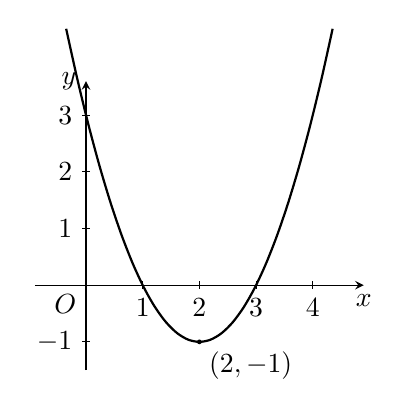
\begin{tikzpicture}[scale=0.72,>=stealth]
  \draw[->] (-0.9,0)--(4.9,0) node[below] {$x$};
  \draw[->] (0,-1.5)--(0,3.6) node[left] {$y$};
  \node[below left] at (0,0) {$O$};
  \foreach \x in {1,2,3,4}{
    \draw[thin] (\x,0.07)--(\x,-0.07) node[below] {$\x$};
  }
  \foreach \y in {-1,1,2,3}{
    \draw[thin] (0.07,\y)--(-0.07,\y) node[left] {$\y$};
  }
  \draw[thick,domain=-0.35:4.35,smooth] plot (\x,{\x*\x-4*\x+3});
  \fill (2,-1) circle (1.2pt);
  \node[below right] at (2,-1) {$(2,-1)$};
\end{tikzpicture}
